\documentclass[11pt]{article}
\usepackage{amsmath,textcomp,amssymb,geometry,graphicx,enumerate,float,mathrsfs}
\graphicspath{{../figures/}}

\def\Name{Jeff Lievense}  % Your name
\def\HW{2} % Homework number

\title{Astronomy 121 -- Spring 2014}
\author{\Name}
\markboth{Astronomy 121 -- Spring 2014, Lab \HW, \Name}{Astronomy 121 -- Spring 2014, Lab \HW, \Name}
\pagestyle{myheadings}

\begin{document}
\maketitle
\begin{center}
{\LARGE {\bf Lab \HW \\~\\ Sampling, Fourier Transforms, Mixers, and Down-Converters}} \\
~\\
~\\
~\\
~\\
~\\
~\\
~\\
\end{center}

\begin{abstract}
    In this report, we develop the necessary theory and tools for designing and implementing digital down-conversion systems. Digital sampling of analog signals is explored, and the Nyquist criterion is established. The spectra of mixed signals are described, and tradeoffs between single- and double-sideband modulation schemes are discussed. We then consider the role of filters in down-conversion and present a simple implementation of an FIR filter on an FPGA.
\end{abstract}

\newpage

\section{Introduction}
In order to use digital signal processing (DSP) techniques to manipulate modulated signals, we must understand the effects of quantizing analog signals and mixing in both time and frequency domains. This involves: understanding how and under what conditions we can sample analog signals; what kind of mixing schemes exist and how we can use DSP to shift desired information to baseband; and how to ensure that we are isolating the desired information, i.e. rejecting useless information that results from mixing. In this lab, we hope to gain a strong understanding of DSP that can be later used in the measurement of the 21-cm line of interstellar atomic hydrogen.

    \subsection{Document Map}
    \begin{itemize}
        \item
            Section 2 discusses necessary background theory.
        \item
            Section 3 describes experimental work carried out in the lab.
        \item
            Sections 4 and 5 discuss the results of our experiments and their consequences.
    \end{itemize}

\section{Theory}
In this section, we discuss the theory used in the development of our system.

    \subsection{Sampling}
    In its most basic form, the Nyquist-Shannon \footnote{http://en.wikipedia.org/wiki/Nyquist\%E2\%80\%93Shannon\_sampling\_theorem\#Why\_Nyquist.3F} sampling theorem states that, if a function $x(t)$ contains no frequencies higher than $B$ hertz, it is completely determined by giving its ordinates at a series of points spaced $\frac{1}{2B}$ seconds apart. In layman's terms, this means that we lose no information in sampling an analog signal if the sampling rate is at least twice the highest frequency present in the signal. This can be seen via a graphical ``proof'' in the frequency domain by looking at sampling as multiplication in time by a Dirac delta train. For those with a taste for linear algebra, it can be shown that bandlimited signals form a subspace of $\mathscr{L}_2(\mathbb{R})$, and we can view sampling mathematically as the projection of a signal onto this space. It can also be shown that the basis for this subspace is a family of sinc functions, and thus we are provided with some insight into the Whittaker-Shannon interpolation formula. \footnote{http://en.wikipedia.org/wiki/Whittaker\%E2\%80\%93Shannon\_interpolation\_formula}
    \\
    \\
    \noindent What occurs as a result of sampling below the Nyquist rate is known as \emph{aliasing}. In general, aliasing describes high-frequency information bleeding into lower frequencies. As we will see in Section 3, when sampling a single sinusoid, aliasing results in the sinusoid becoming indistinguishable from lower frequency sinusoids. This of course is a very undesirable property in a down-conversion system, therefore we must pay careful attention to the bandlimited-ness of our signals and how we sample them.

    \subsection{Mixing}
    In general, mixing refers to multiplication of a signal by a sinusoid in order to shift its spectrum from one frequency range to another. This process is also known as \emph{heterodyning}. In this lab, we are interested in mixing for its use in \emph{down-conversion}, that is, shifting some signal of interest from a high frequency range a lower intermediate frequency range (IF) or baseband (low frequency, centered around DC). \\
    \\
    In the ideal mathematical case, mixing a signal with a complex exponential shifts the signal's spectrum to be centered around the frequency of the complex exponential. This can be seen via the \emph{modulation property} (a result of the \emph{Convolution Theorem}) of the Fourier transform:
    \begin{flalign*}
        x(t)e^{j\omega_0 t} &\overset{\mathcal{F}}{\leftrightarrow} X(j(\omega - \omega_0)),
    \end{flalign*}
    where $x(t)$ is the signal of interest, $X(j\omega)$ is its spectrum, and $\mathcal{F}$ denotes a Fourier transform pair. Unfortunately, complex exponentials cannot be generated in hardware for actual mixing purposes, so the mixing sinusoid is more often a cosine. In this case, the spectrum of $x(t)$ is shifted both positive and negative frequencies. Using the Fourier series expansion $\cos(\omega_0 t) = \frac{1}{2}e^{j\omega_0 t} + \frac{1}{2}e^{-j\omega_0 t}$ and the linearity of the Fourier transform, we see that
    \begin{flalign*}
        x(t)\cos(\omega_0 t) &\overset{\mathcal{F}}{\leftrightarrow} \frac{1}{2}X(j(\omega - \omega_0)) + \frac{1}{2}X(j(\omega + \omega_0)).
    \end{flalign*}
    This kind of modulation is known as \emph{double-sideband modulation} (DSB). We note that there is redundancy in the modulated signal -- provided that $\omega_0$ is large enough to prevent aliasing, $X(j\omega)$ occurs twice in the above expression! To save transmission power and frequency occupancy (bandwidth), \emph{single-sideband modulation} (SSB) can be used instead. This concept will be explored in Section 3.

    \subsection{Down-Conversion}
    As mentioned above, our ultimate goal in this lab is to design a \emph{down-conversion} system. This entails extracting information from a modulated signal by shifting the spectrum down to baseband and removing high frequency artifacts left over from mixing (namely the sum frequency), thus we require the use of a low-pass filter. The theory of analog filters was described in the last lab, but we are now interesting in performing filtering digitally. To accomplish this, we will design filters by specifying their frequency response, then determining the necessary impulse response by taking an inverse discrete Fourier transform (DFT). The nonzero values of the impulse response will hence be referred to as the \emph{filter coefficients} which can be used to filter a signal via convolution. Since convolution consists of basic operations (multiplying, adding, shifting), we can efficiently implement our desired filter on an \emph{field programmable gate array} (FPGA).

\section{Methods}
In this section we discuss the verification and physical implementation of the theory discussed above.

\begin{figure}[H]
    \centering
        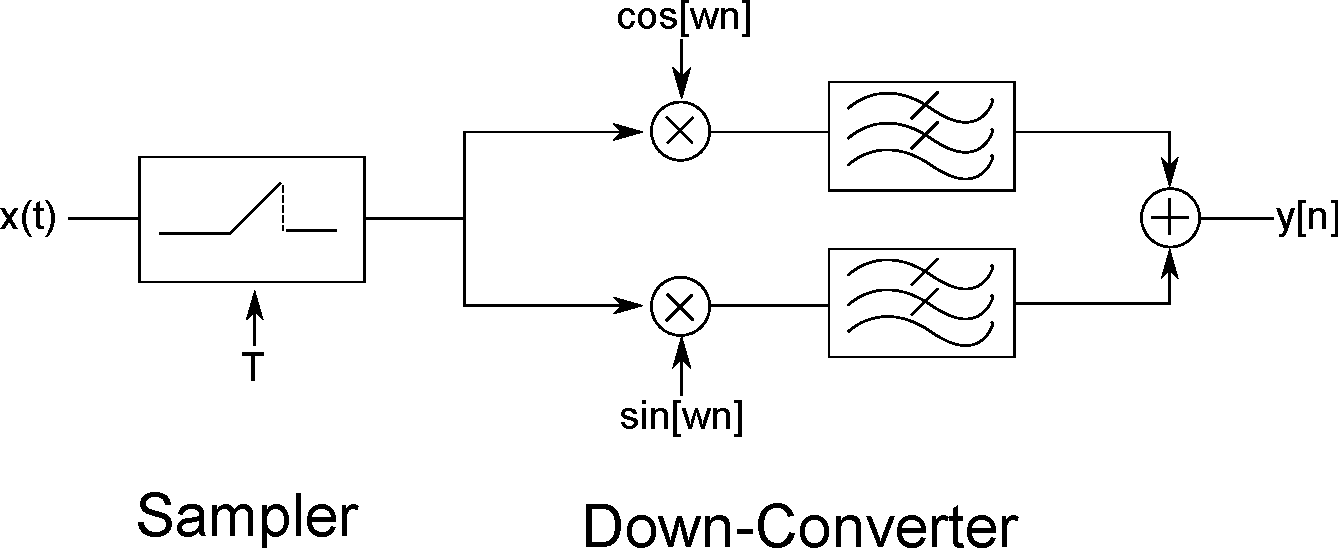
\includegraphics[width = \textwidth]{down-converter.pdf}
    \caption{Overall digital down-converter system.}
    \label{bd}
\end{figure}

    \subsection{Overview}
    We are interested in combining the concepts discussed in previous sections in order to realize a complete digital down-conversion system. Figure~\ref{bd} presents a block diagram of what our circuit should do:
    \begin{itemize}
        \item Sampling
        \item Mixing
        \item Filtering
    \end{itemize}

    \subsection{Observing the Nyquist Criterion}
    To solidify our understanding of the sampling theorem, we consider the following system, where the continuous time signal $x(t) = \cos(2\pi v_{\text{sig}})$ is sampled with sampling period $T = \frac{1}{v_{\text{smpl}}}$ to yield the discrete time signal $x[n]$:
    \begin{figure}[H]
        \centering
            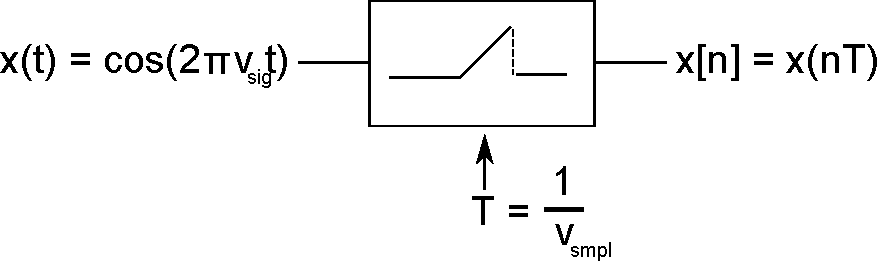
\includegraphics[width = \textwidth]{sampler.pdf}
        \caption{A sampler with sampling period $T$ [s] and sampling rate $v_{\text{smpl}}$ [Hz].}
    \end{figure}
    \noindent The Nyquist criterion asserts $v_{\text{smpl}} \geq 2v_{\text{sig}} \Rightarrow \alpha = \frac{v_{\text{sig}}}{v_{\text{smpl}}} \leq 0.5$ in order for $x(t)$ to be completely determined by its samples $x[n]$. To verify this, we try sampling with $\alpha = 0.1, 0.2, \dotsc, 0.8, 0.9$. As seen below in Figure~\ref{nyquist}, when $\alpha = 0.1$ sufficiently clears the Nyquist criterion, we are provided with an accurate sampled representation of $x(t)$. This continues to hold until we reach the limiting case in which $\alpha = 0.5$. We see that, using a sampling rate of $v_{\text{smpl}}$, the highest frequency we can completely determine from its samples is $v_{\text{sig}} = \frac{v_{\text{smpl}}}{2}$ -- since $x[n]$ is a discrete time signal (its domain is $\mathbb{Z}$), the smallest possible period (which corresponds to the highest possible frequency) is 2 samples, and we see this is achieved when $\alpha = 0.5$. As $\alpha$ increases from 0.5 to 0.9 (i.e. as $v_{\text{sig}}$ increases), we observe a very interesting phenomenon: the frequency of $x[n]$ \emph{decreases}! In fact, when $\alpha = 0.9$, $x[n]$ has roughly the same frequency as it did when $\alpha = 0.1$, even though the frequency of the continuous time signal $x(t)$ we are sampling has increased by a factor of 9 (see Figure~\ref{nyquist}). This is aliasing in action.
    \begin{figure}[H]
        \centering
            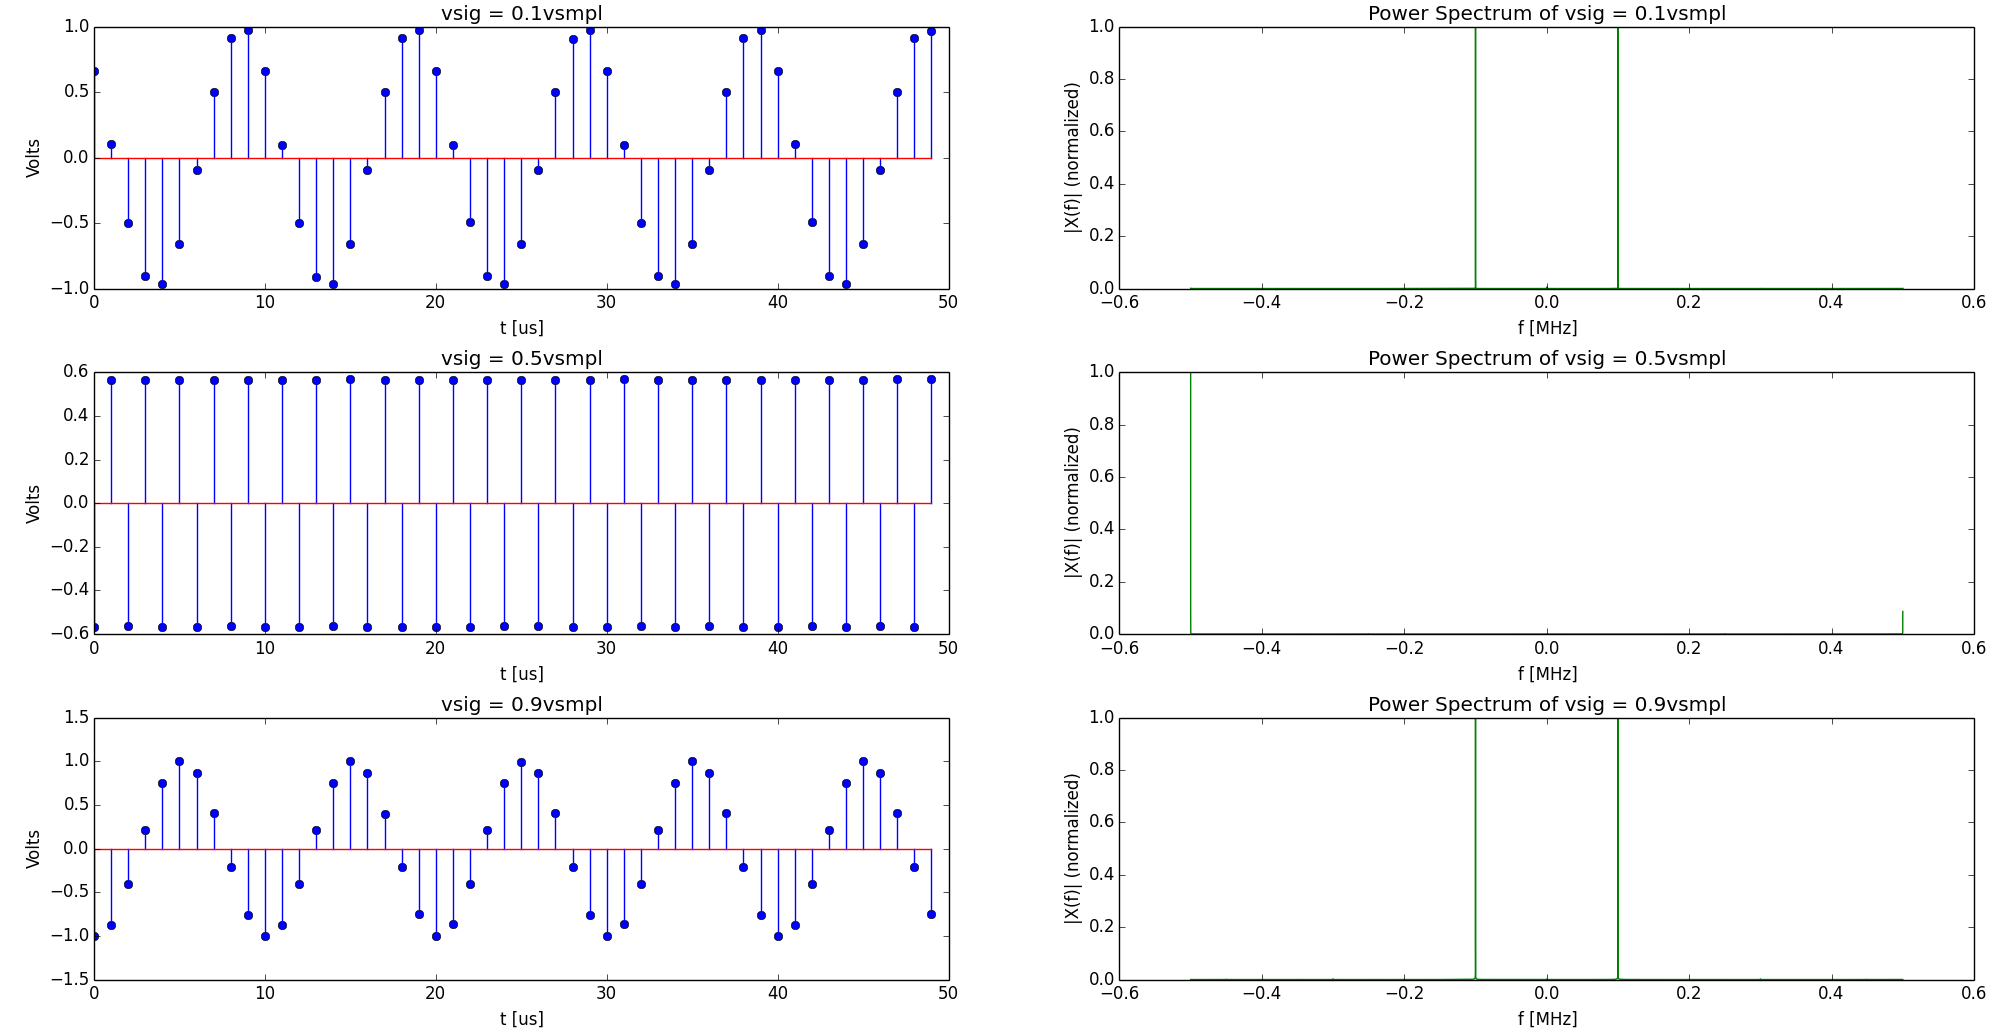
\includegraphics[width = \textwidth]{1_3_sampling.png}
        \caption{Sampling a sinusoid below, at, and above the Nyquist rate.}
        \label{nyquist}
    \end{figure}


    \subsection{Mixing \& Sidebands}
    We now investigate analog and digital mixers. In the lab, we have at our disposal an analog DSB mixer, a digital DSB mixer which multiplies a provided signal by a provided local oscillator (LO) signal, and a digital SSB mixer which multiplies a provided signal by an on-board LO signal.
    
    \noindent Figure~\ref{dsbfilt} shows the power spectra of two signals, with frequencies $v_{\text{sig}} = v_{\text{LO}} \pm \delta_f$, at the output of the analog DSB mixer. Note that there is symmetry about the sum and difference frequencies: this is DSB modulation. The \emph{upper sideband} (USB, spectral content at frequencies with greater magnitude than the carrier) and \emph{lower sideband} (LSB, spectral content at frequencies with lesser magnitude than the carrier) are mirror images of each other. Additionally shown is the output waveform for $\delta_f = .05\cdot v_{\text{LO}}$. We are interested in the low frequency signal which is clearly present, but is corrupt with a high frequency (the sum frequency) signal. To solve this, we use a digital low-pass filter to remove the sum frequencies by zeroing out the high frequency DFT coefficients of the signal. The result is shown next to the original output, and we see the low frequency signal in its unaltered state.
    
    \begin{figure}[H]
        \centering
            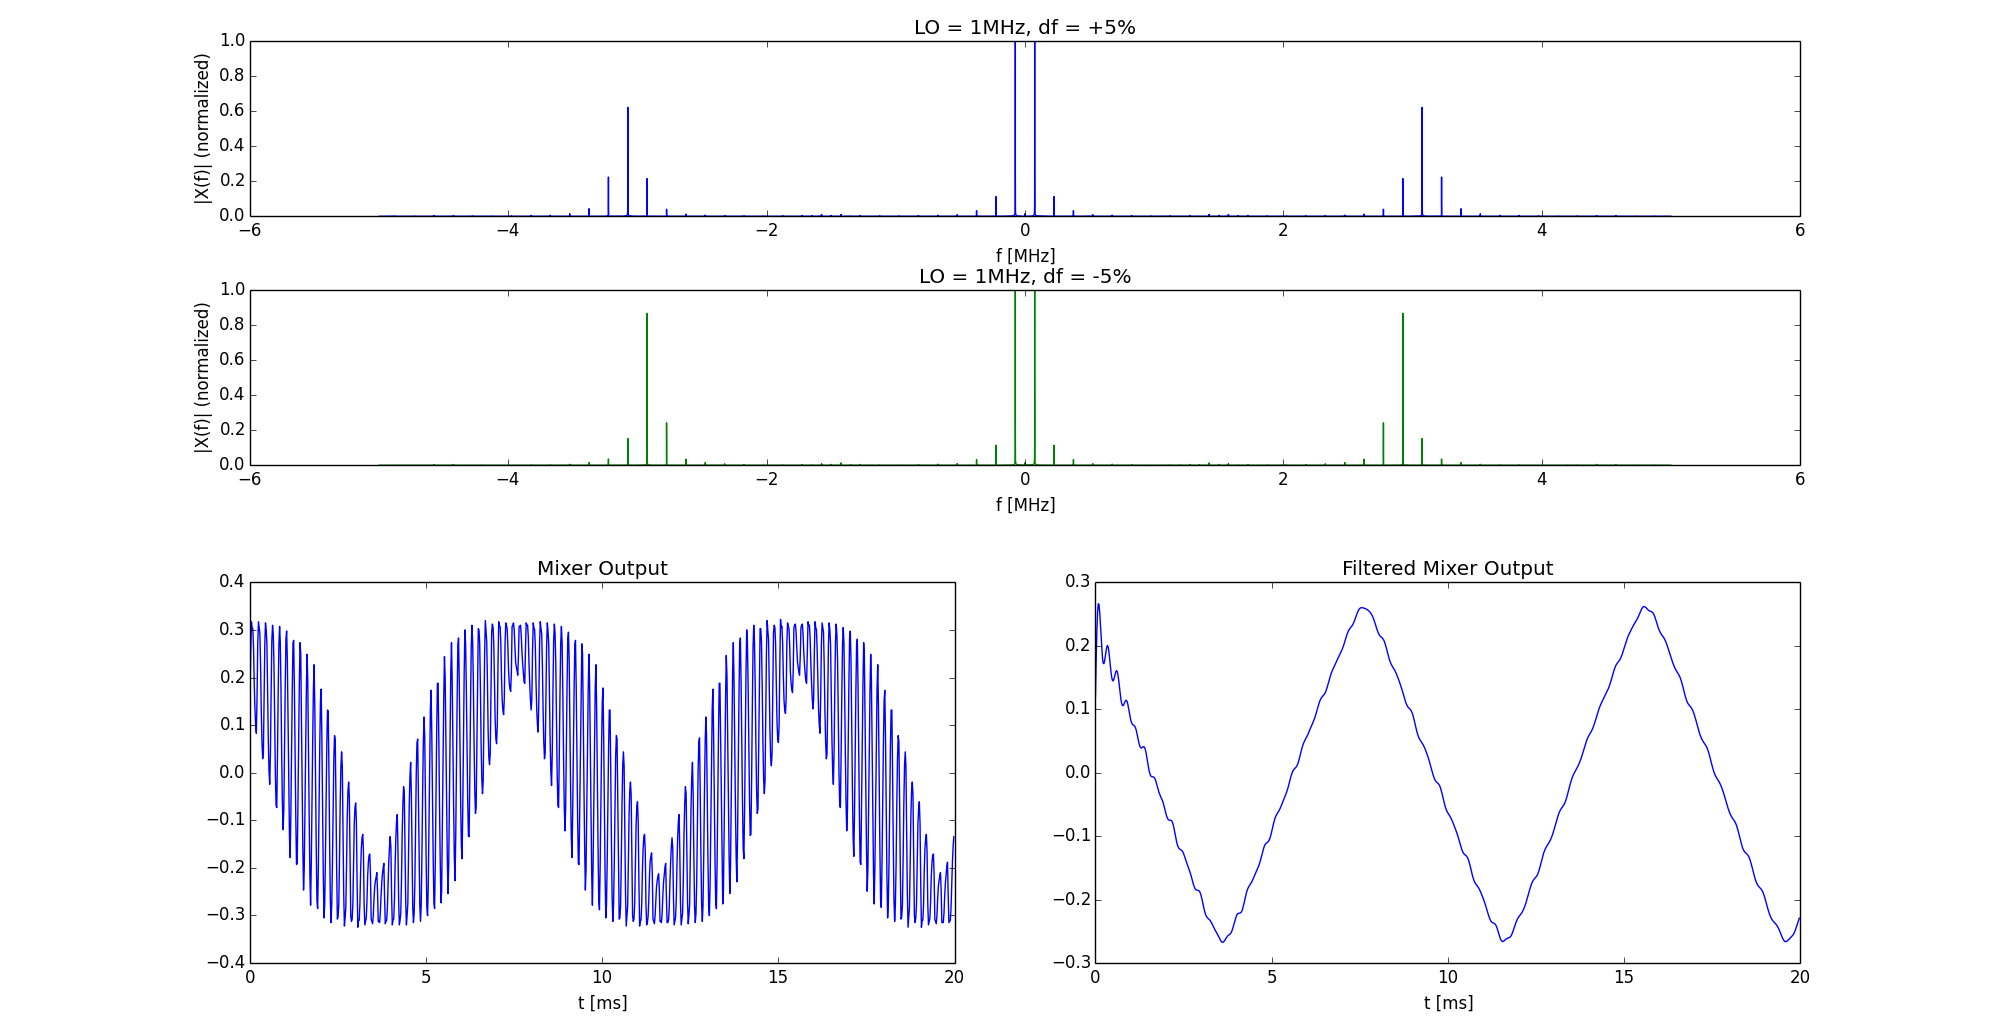
\includegraphics[width = \textwidth]{2_1_2_filtering.png}
        \caption{DSB power spectra and filtered mixer output.}
        \label{dsbfilt}
    \end{figure}
    
    \noindent Figure~\ref{sbfreq} shows various power spectra: two signals with frequencies $v_{\text{sig}} = v_{\text{LO}} \pm \delta_f$ at the output of the digital DSB mixer; one at the output of the digital SSB mixer; and the individual components of the digital SSB mixer output ($I$, the \emph{in-phase} component, i.e. mixed with cosine; $Q$, the \emph{quadrature} component, i.e. mixed with sine). It is here that we see the difference between DSB and SSB mixing: whereas DSB mixing/down-conversion is performed by multiplying the signal by a single cosine and filtering, SSB mixing/down-conversion involves splitting the signal, multiplying by both cosine and sine to yield $I(t)$ and $Q(t)$ (respectively), composing a new signal $y(t) = I(t) + jQ(t)$, and then filtering. More formally, if the signal to be down-converted is $x(t)$, we have (in discrete time domain, after $x(t)$ has been sampled to yield $x[n]$)
    \begin{flalign*}
        I[n] &= \cos(\omega_0 n)x[n] \overset{\mathcal{F}}{\leftrightarrow} \frac{1}{2}(X(e^{j(\omega - \omega_0)}) + X(e^{j(\omega + \omega_0)}) \\
        Q[n] &= \sin(\omega_0 n)x[n] \overset{\mathcal{F}}{\leftrightarrow} \frac{1}{2j}(X(e^{j(\omega - \omega_0)}) - X(e^{j(\omega + \omega_0)}) \\
        Y(e^{j\omega}) &= I(n) + jQ(n) \\
        &=  \frac{1}{2}(X(e^{j(\omega - \omega_0)}) + X(e^{j(\omega + \omega_0)}) + j\frac{1}{2j}(X(e^{j(\omega - \omega_0)}) - X(e^{j(\omega + \omega_0)}) \\
        &= X(e^{j(\omega - \omega_0)}),
    \end{flalign*}
    and therefore we see SSB mixing yields the down-converted signal with much less spectral occupancy than DSB mixing. In Figure~\ref{sbfreq}, we see that the reconstructed SSB mixed signal only contains the USB of the $I$ and $Q$ signals. In Figure~\ref{ssbtime}, we see the real and imaginary parts ($I[n]$, $jQ[n]$) of the output SSB mixer and the filtered output.

    \begin{figure}[H]
        \centering
            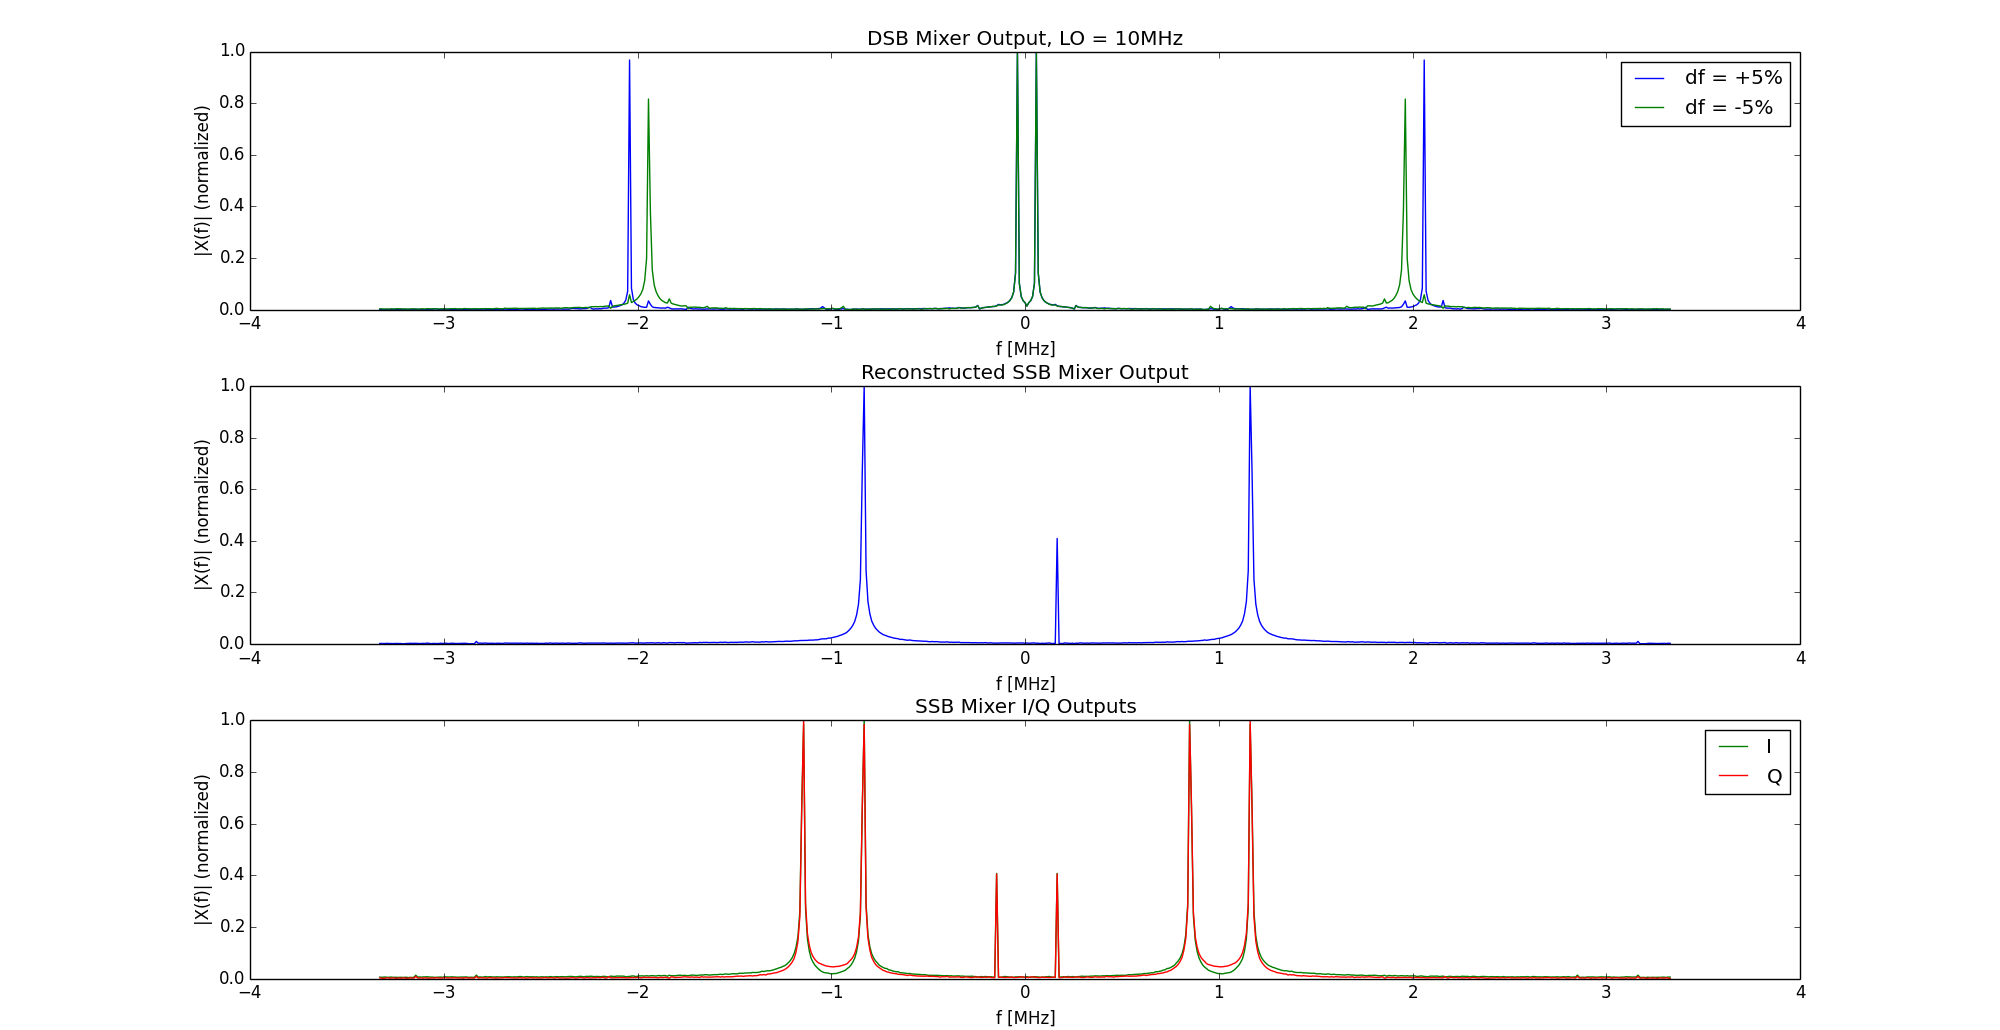
\includegraphics[width = \textwidth]{2_2_2_dsb_ssb_freq.png}
        \caption{DSB and SSB power spectra.}
        \label{sbfreq}
    \end{figure}

    \begin{figure}[H]
        \centering
            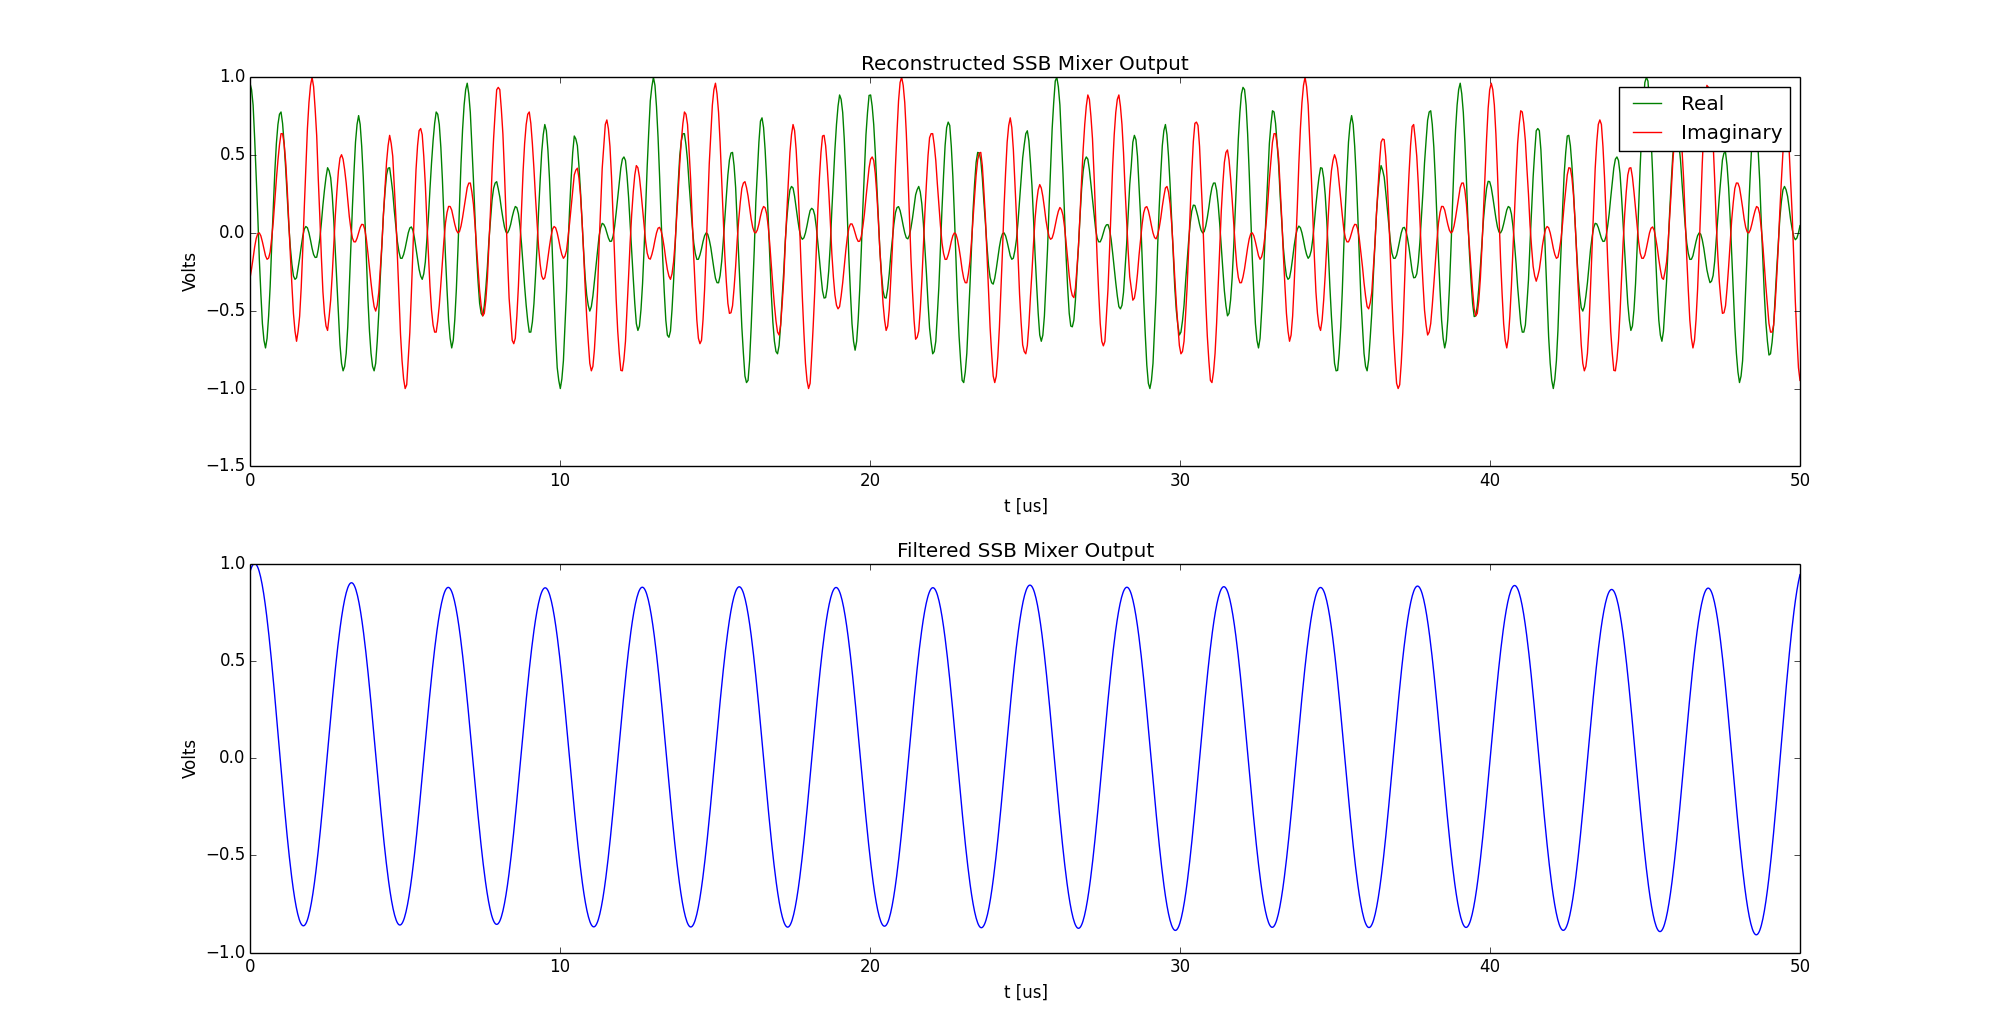
\includegraphics[width = \textwidth]{2_2_2_ssb_time.png}
        \caption{Reconstructing a signal from the complex outputs of a SSB mixer.}
        \label{ssbtime}
    \end{figure}
    
    As mentioned about, SSB is more efficient than DSB -- there is less redundancy in the modulated signal, therefore it takes less transmitter power and occupies less spectral real estate (which is very expensive!). Another consideration is analog vs. digital. To understand the advantage of a digital implementation, we need to take a step back and look at the bigger picture. In a real communication system (see Figure~\ref{commsys}), our signal of interest $x(t)$ is actually an up-converted version of some message signal $m(t)$, i.e. $x(t) = m(t)\cos(\omega_0 t)$. We would then like to transmit $x(t)$ across some channel and down-convert it at the receiver to recover $m(t)$. As we've found in this lab, down-converting $x(t)$ means mixing with $\cos(\omega_0 t)$ then filtering. In an analog system, the LOs at the transmitter and receiver are implemented in hardware, and as one can imagine, it is hard to ensure these oscillators in separate locations are exactly in phase. We can model this problem by adding a phase shift $\phi$ to the receiver LO relative to the transmitter LO:
    
    \begin{figure}[H]
        \centering
            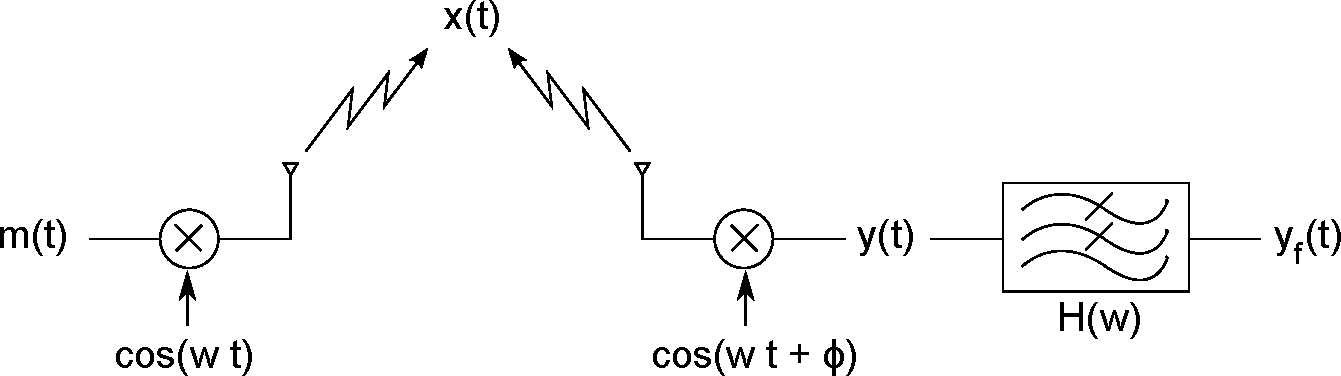
\includegraphics[width = \textwidth]{commsys.pdf}
        \caption{A simplified DSB-AM communication system.}
        \label{commsys}
    \end{figure}
    
    Mathematically, we have
    \begin{flalign*}
        y(t) &= \cos(\omega_0 t + \phi)x(t) \\
        &= \cos(\omega_0 t + \phi)\cos(\omega_0 t)m(t) \\
        &= \frac{1}{2}(\cos(2\omega_0 t + \phi) + \cos(\phi))m(t),
    \end{flalign*}
    and after filtering out the sum frequency via an appropriately chosen filter $H(\omega)$, we have
    \begin{flalign*}
        y_f(t) &= \frac{cos(\phi)}{2}m(t).
    \end{flalign*}
    This is not the signal we are trying to recover! Since $\phi$ can be modeled as a random variable ($\phi\sim U[-\pi,\pi]$), the receiver will have a hard time determining what the message $m(t)$ actually is. Thus it is clear that a digital implementation of such a system is preferred, since the LO signals can be precisely generated in phase.


    \subsection{Filtering}
    The final stage in our digital down-conversion is the low-pass filter. As mentioned previously, we will design this filter $H$ in the frequency domain by specifying the desired frequency response $H_k$, then take an inverse DFT to find the time domain coefficients $h_n$ which we will convolve our input signals with to achieve the filtering. The desired frequency response in array form is
    \begin{flalign*}
        &\begin{bmatrix} H_0 & H_1 & H_2 & H_3 & H_4 & H_5 & H_6 & H_7 \end{bmatrix} = \\
        &\begin{bmatrix} 1 & 1 & 1 & 0 & 0 & 0 & 1 & 1 \end{bmatrix},
    \end{flalign*}
    and via Python's \texttt{fft} module, we see that the necessary coefficients are
    \begin{flalign*}
        &\begin{bmatrix} h_0 & h_1 & h_2 & h_3 & h_4 & h_5 & h_6 & h_7 \end{bmatrix} = \\
        &\begin{bmatrix} 0.625 & 0.3017767 & -0.125 & -0.0517767 & 0.125 & -0.0517767 & -0.125 & 0.3017767 \end{bmatrix}.
    \end{flalign*}
    
    \noindent The FPGA which will implement our filter needs the coefficients to be written as fixed-point numbers. Assuming that software registers will be interpreted on the FPGA as 18-bit signed integers with 17 bits after the binary point, we have: \\
    \\
    \begin{center}
        \begin{tabular}{| l || l|}
            \hline
            Coefficient & Fixed-Point Representation \\ \hline
            $h_0$ & 0.10100000000000000 \\
            $h_1$ & 0.01001101010000010 \\
            $h_2$ & 1.11100000000000000 \\
            $h_3$ & 1.11110010101111110 \\
            $h_4$ & 0.00100000000000000 \\
            $h_5$ & 1.11110010101111110 \\
            $h_6$ & 1.11100000000000000 \\
            $h_7$ & 0.01001101010000010 \\
            \hline
        \end{tabular}
    \end{center}

    We then implement this filter on the FPGA and determine the actual shape of the filter empirically. This is done by inputting a series of sinusoids at different frequencies and measuring the gain of the filter at each frequency. By definition, this is measuring the frequency response of the filter.  Figure~\ref{filter} shows the samples of the frequency response determined empirically in addition to the calculated frequency response of the zero-padded coefficients and the ideal filter:
    
    \noindent 
    \begin{figure}[H]
        \centering
            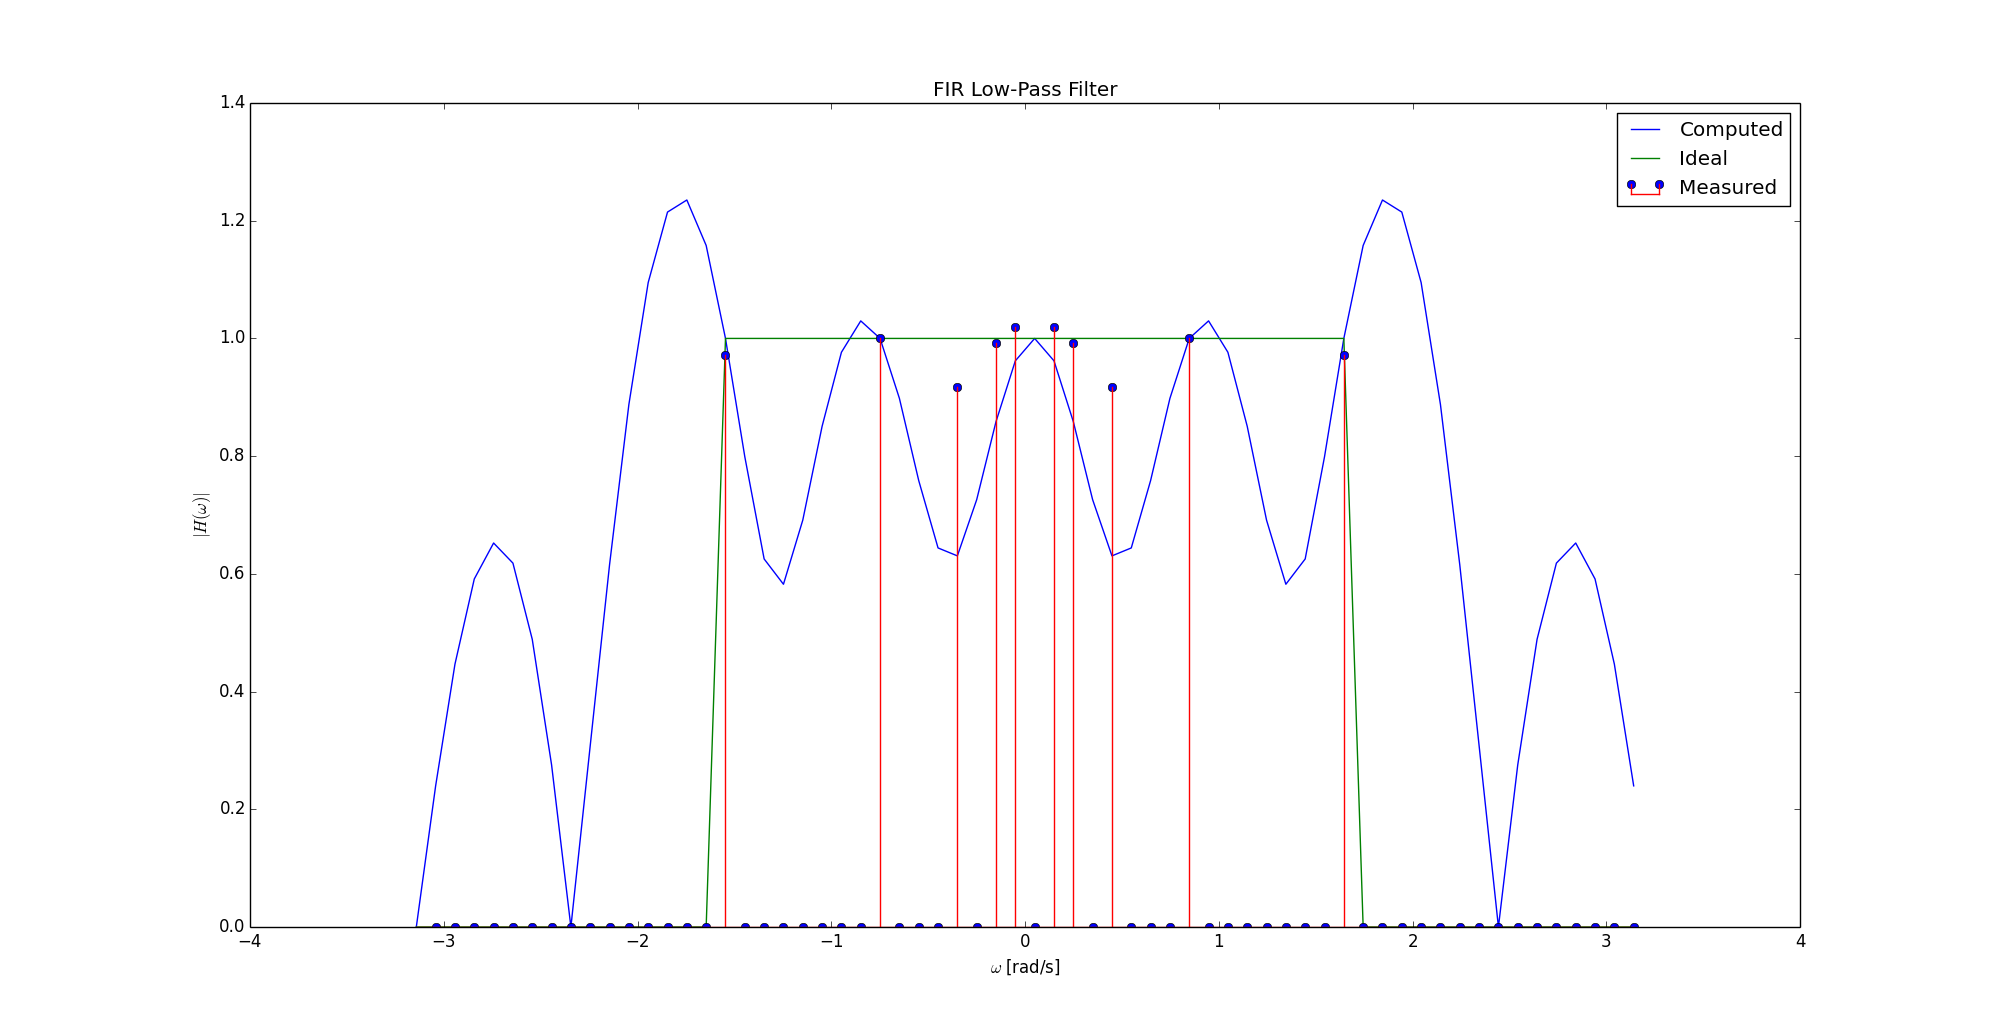
\includegraphics[width = \textwidth]{3_2_1_filter.png}
        \caption{Comparison of ideal, computed, and empirically determined filter shapes.}
        \label{filter}
    \end{figure}
    
    


\section{Results \& Discussion}


\section{Conclusion}


\section{Acknowledgements}
We would like to thank: Isaac Domagalski and Eduardo Herrera for their help in carrying out the work described above; Baylee Bordwell and Garret ``Karto'' Keating for their assistance; and Aaron Parsons for providing the opportunity and facilities necessary to perform these experiments.

\end{document}
